\documentclass[]{report}

\usepackage[utf8]{inputenc}
\usepackage{natbib}

\usepackage{graphicx}
\usepackage{amsmath}
\usepackage{amsfonts}
\usepackage{xfrac}
\usepackage{subfigure}
\usepackage{url}
\usepackage{epigraph}
\usepackage{csquotes}

\usepackage{listings}
\usepackage{color}

\definecolor{dkgreen}{rgb}{0,0.6,0}
\definecolor{gray}{rgb}{0.5,0.5,0.5}
\definecolor{mauve}{rgb}{0.58,0,0.82}

\lstset{frame=tb,
	language=Java,
	aboveskip=3mm,
	belowskip=3mm,
	showstringspaces=false,
	columns=flexible,
	basicstyle={\small\ttfamily},
	numbers=none,
	numberstyle=\tiny\color{gray},
	keywordstyle=\color{blue},
	commentstyle=\color{dkgreen},
	stringstyle=\color{mauve},
	breaklines=true,
	breakatwhitespace=true,
	tabsize=3
}

% Title Page
\title{A Geometric Constraint Engine \\
	The Freed Linkage Assembler (FLA)}
\author{Fredrick P. Eisele}
\date{2014 December 12}

\begin{document}
	\maketitle
	
	\begin{abstract}
		It is a fact that modern engineering and manufacturing operate in an environment of heterogeneous protocols, many of them closed. 
		CyPhy positions itself at the intersection of these tools and their work products. 
		CyPhy defines higher-level objects by applying constraints between the work products. 
		The solution to these constraints establishes the design space of component assemblies. 
		There are several open-source offerings which provide component design, but lack component assembly. 
		Most commercial component assembly is embedded in closed-source CAD systems. 
		Prior META effort has been to make use of these commercial assemblers to demonstrate feasibility.  
		As part of this effort, the most capable open-source CAD packages available today were evaluated, 
		but unfortunately none had a geometric constraint solver capable of structurally 
		composing CyPhy designs comparable to the success we had with commercial offerings (i.e. Creo).  
		To this end, the freed-linkage-assembler 
		(FLA \footnote{This is a Vanderbilt open-source project \url{https://github.com/phreed/freed-linkage-assembler}.}) 
		is a Java virtual machine 
		executable written by Vanderbilt as an open-source software. 
		This program solves the geometric constraint problem specified in CyPhy and 
		produces a set of metric preserving translations and rotations (i.e. versors) over the assembly’s components. 
		This artifact is useful to the designer and is critical in the analysis of assemblies. 
		As a side benefit, the complexity of assembly is a good match with design complexity.

	\end{abstract}

\chapter{Motivation}

\epigraph{Because primarily of the power of the Internet, 
people of modest means can band together and amass 
vast sums of money that can change the world 
for some public good if they all agree.}{William J. Clinton}

\begin{figure}[h!]
	\centering
	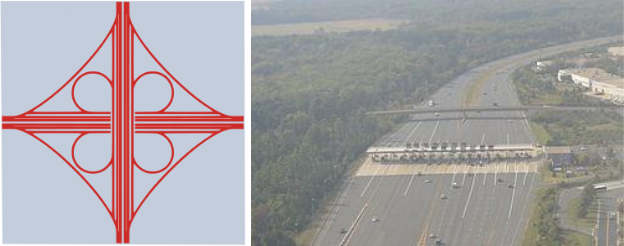
\includegraphics[scale=0.7]{images/image07}
	\caption{Open Systems can improve flow.  Closed systems restrict flow.}
	\label{fig:open-or-restrict-flow}
\end{figure}

The primary goal of the geometric constraint engine is to demonstrate the feasibility of an open-source assembly composition. In particular, to support those constraints required for the program projects. A secondary goal is to provide an unambiguous complexity measure and a means for augmenting the system to allow for assembly of greater complexity.

\section{Objective}

The purpose of this software, FLA,  is to provide an open-source alternative to commercial and proprietary offerings, 
an entry and exit ramp to the structural design freeway that is CyPhy.  
Generally, the problem addressed here is the same as that of the CAD Assembler (CreateAssembly Program),
namely, to eliminate the  manual building of CAD assemblies, replacing it with automation.
While executing the AVM program and using the assembly programs embedded in CAD packages, 
it was discovered that they are not constructed to work in an automatic fashion; rather, 
they presume the presence of an operator who will “revert to manual” to resolve the numerical glitches. 
The knowledge contributed by the operator is used, but not retained in the model, nor in the assembler. 
A goal of this product is to enable fully automatic regeneration of assemblies from design constraints.
The CyPhy tools present a way that uses less geometry to 
express joints between components to constrain assemblies. 
The current tools rely on Creo Parametric, a commercial CAD package, for 3D CAD model assembly composition. 
This task will augment the existing component interface to carry placement objects, known as versors. 
A representative open-source CAD platform will be selected as the target for composition. 
The most significant part of this task was the development of a geometric constraint solver, which current open-source CAD tools lack. 

\begin{figure}[h!]
	\centering
	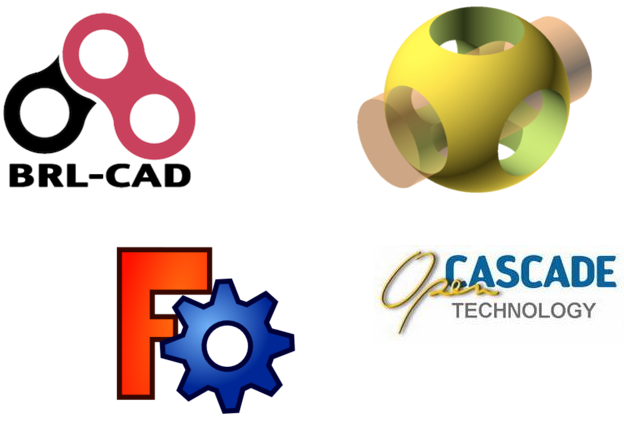
\includegraphics[scale=0.7]{images/image11.png}
	\caption{A representative sample of the open-source CAD systems}
	\label{fig:foss-cad}
\end{figure}

Several open-source CAD systems were evaluated as possible targets.  
Each was found to have suitable means for visualizing assembles and for loading and placement. 
The packages we evaluated extensively and their mechanisms evaluated are: 
OpenCascade \footnote{\url{http://www.opencascade.org/}}, a geometric model library; 
BRL-CAD \footnote{\url{http://brlcad.org/}}; and 
OpenSCAD \footnote{\url{http://www.openscad.org/}}. 
OpenCascade has more than one third-party interactive interface, 
FreeCAD \footnote{\url{http://sourceforge.net/projects/free-cad}} and
NaroCAD \footnote{\url{http://narocad.com/}}. 
OpenCascade has mechanisms for loading STEP files into a feature tree along with placement. 
It also has an API which is expressed in several programming languages: 
Python, Java, Tcl and C++. BRL-CAD and OpenSCAD models are both updated 
through textual interfaces, which makes them suitable for automatic control.  
BRL-CAD and OpenCascade can read many formats, including STEP and STL; 
OpenSCAD can import STL files.  
Due to its lightweight footprint and availability in browsers 
\footnote{\url{http://openjscad.org/}}
OpenSCAD was selected as the primary target visualization environment.

\section{Data Flow}

The demonstration environment in which the FLA is operating is 
a modification that has been developed for CreateAssembly. 
FLA receives its input geometric constraints from the CyPhy2CAD 
interpreter and produces a composed geometry that is output to CreateAssembly and others.  
It augments the \texttt{CADAssembly.xml} file with component positions 
and creates files used for geometry visualization. 
The implemented sequential approach is depicted in Fig. Assembly Composition Process. 
The \texttt{CAD\_Assembly.xml} file is produced by CyPhy2CAD.  

\begin{figure}[h!]
	\centering
	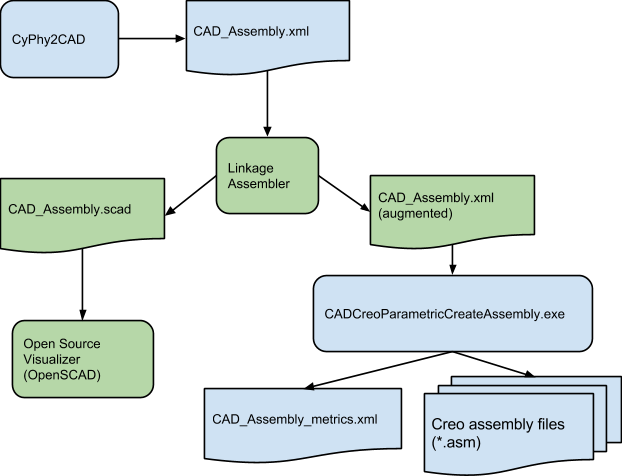
\includegraphics[scale=0.7]{images/image13}
	\caption{Assembly Composition Process}
	\label{fig:assy-compose}
\end{figure}

\subsection{Inputs}

FLA requires that the geometry of the component interfaces be included in the curated component meta-data.  
This supplemental marker geometry is placed in the \texttt{CAD\_Assembly.xml} file by CyPhy2CAD.  
The supplemental geometry represents the component datum objects as well as the constraints.

\begin{figure}
\begin{lstlisting}
<?xml version="1.0" encoding="utf-8"?>
<Assemblies  
    xmlns:xsi="http://www.w3.org/2001/XMLSchema-instance" 
    xmlns:xsd="http://www.w3.org/2001/XMLSchema" VersionInfo=""     
    xsi:noNamespaceSchemaLocation="AssemblyInterface.xsd">
  <Assembly ConfigurationID="{ASSY}" _id="id1">
    <CADComponent  
        ComponentID="{ASSY}" 
        Name="ComponentAssembly_1"
        DisplayName="ComponentAssembly_1" Type="ASSEMBLY"
        SpecialInstruction="" MaterialID="" Representation=""
       _id="id2">
     <CADComponent 
         ComponentID="{BAR-1}" 
         Name="BAR_1" DisplayName="Bar_1"
         Type="PART" SpecialInstruction="" MaterialID=""
         Representation=""
         Classification="Unknown" _id="id21">
       <Constraint _id="id27">
         <Pair FeatureInterfaceType="CAD_DATUM"
               FeatureGeometryType="SURFACE"           
               FeatureAlignmentType="ALIGN" _id="id28">
           <ConstraintFeature 
               ComponentID="{BAR-1}" 
               FeatureName="FRONT"
               FeatureOrientationType="SIDE_A" _id="id29">
            <GeometryMarker 
                 x="0" y="0" z="0" 
                 i="0" j="0" k="1" pi="0" _id="id30" />
          </ConstraintFeature> ...
\end{lstlisting}
\caption{\texttt{CAD\_Assembly.xml} (from CyPhy)}
\end{figure}



\subsection{Outputs} 

The \texttt{CAD\_Assembly.xml} file is augmented by the assembler, which is a geometric constraint solver.  
It augments the XML file with transformation objects, versors, 
which specify the location, orientation and rotation of the components.
This additional information is:
necessary for CAD systems which do not have a constraint based assembler, and
useful for providing an initial configuration to CAD systems that use numerical constraint engines.


\begin{figure}
	\begin{lstlisting}
<?xml version="1.0" encoding="utf-8"?>
<Assemblies  
    xmlns:xsi="http://www.w3.org/2001/XMLSchema-instance" 
    xmlns:xsd="http://www.w3.org/2001/XMLSchema" VersionInfo=""     
    xsi:noNamespaceSchemaLocation="AssemblyInterface.xsd">
  <Assembly ConfigurationID="{ASSY}" _id="id1">
    <CADComponent  
        ComponentID="{ASSY}" 
        Name="ComponentAssembly_1"
        DisplayName="ComponentAssembly_1" Type="ASSEMBLY"
        SpecialInstruction="" MaterialID="" Representation=""
       _id="id2">
      <versor x="0.0" y="0.0" z="0.0" 
          pi="0.0" i="0.0" j="0.0" k="0.0"/>
      <CADComponent 
          ComponentID="{BAR-1}" 
          Name="BAR_1" DisplayName="Bar_1"
          Type="PART" SpecialInstruction="" MaterialID=""
          Representation=""
          Classification="Unknown" _id="id21">
        <versor x="12315.409884054143" 
                y="-4259.980462767625"
                z="903.0008418651848" 
                pi="9.86929044315234" 
                i="-0.8894325067015925" 
                j="0.4570665300942336"  
                k="-2.435861248047122E-5"/>
       <Constraint _id="id27">
         <Pair FeatureInterfaceType="CAD_DATUM"
               FeatureGeometryType="SURFACE"           
               FeatureAlignmentType="ALIGN" _id="id28">
          <ConstraintFeature 
                 ComponentID="{BAR-1}" 
                 FeatureName="FRONT"
                 FeatureOrientationType="SIDE_A" _id="id29">
            <GeometryMarker 
                   x="0" y="0" z="0" 
                   i="0" j="0" k="1" pi="0" _id="id30" />
          </ConstraintFeature> 
\end{lstlisting}
\caption{CyPhy Output file augmented with versors}
\end{figure}

\begin{figure}
	\begin{lstlisting}
	
translate ([0.0, 0.0, 0.0]) {
  rotate (a=0.0, v=[0.0, 0.0, 0.0]) {
    import ("BAR_1.stl"); }}

translate ([50.000, 49.99999, 0.0]) {
  rotate (a=180.0, 
          v=[-0.7071067811865475, 
             -0.7071067811865476, 
             -4.329780281177466E-17]) {
    import ("BAR_1.stl"); }}

translate ([100.000, 99.999, 0.0]) {
  rotate (a=0.0, v=[0.0, 0.0, 0.0]) {
    import ("BAR_1.stl"); }}

translate ([150.00000000000017, 150.0, 0.0]) {
  rotate (a=180.0, 
          v=[-0.7071067811865475, 
             -0.7071067811865476,
             -4.329780281177466E-17]) {
    import ("BAR_1.stl"); }}
\end{lstlisting}
\caption{OpenSCAD Input : 4Bar Sample}
\end{figure}


The OpenSCAD file consists of a set of components and their placement. 
The components are imported stereolithography files (*.stl), 
which are then rotated and translated into their proper positions. 
The linkage assembler computes these rotations and translations from the constraints. 
The linkage also produces an assembly plan, an ordered list of 
the functions and the constraints which they satisfy. 
This linkage assembly plan is itself an important artifact
\footnote{\url{Not yet written to a file by FLA.}} 
that is not exposed by commercial CAD products.

\section{Detailed Description}

The FLA is a constraint solver that finds solutions to a set of geometric constraints.

\subsection{Open-Source Replacement}

The block diagram (<Fig. Assembly Composition Process>) shows that 
the FLA reads the output from CyPhy2CAD and augments it with versors. 
Constraints may be strict or guides. Strict constraints must be met as specified; 
if they are not met, this indicates a defect in the assembly specification. 
Over-constrained and under-constrained systems are allowed. 
Guide constraints are recruited as needed to obtain a single 
solution to a constraint set. We anticipate other geometric 
items will be introduced to support future solution functions. 
In general, the operator process is identical to that of the CreateAssembly Program. 
A CyPhy model is created with its attendant joint constraints. 
These constraints represent a set of restrictions on the design assembly. 
The successful application of FLA results in a well formed design assembly of component parts. 

\begin{figure}[ht!]
	\centering
	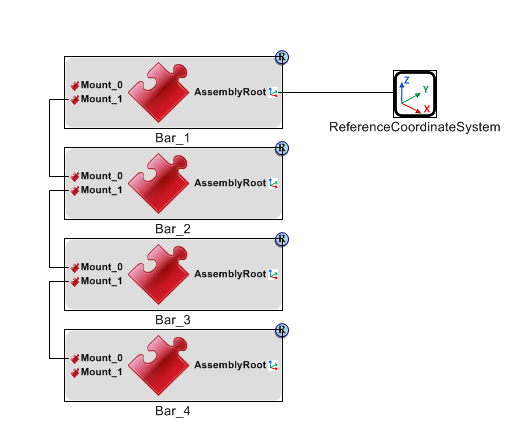
\includegraphics[scale=0.7]{images/image00.png}
	\caption{CyPhy View : 4Bar Sample}
	\label{fig:4bar-cyphy}
\end{figure}


\begin{figure}[ht!]
	\centering
	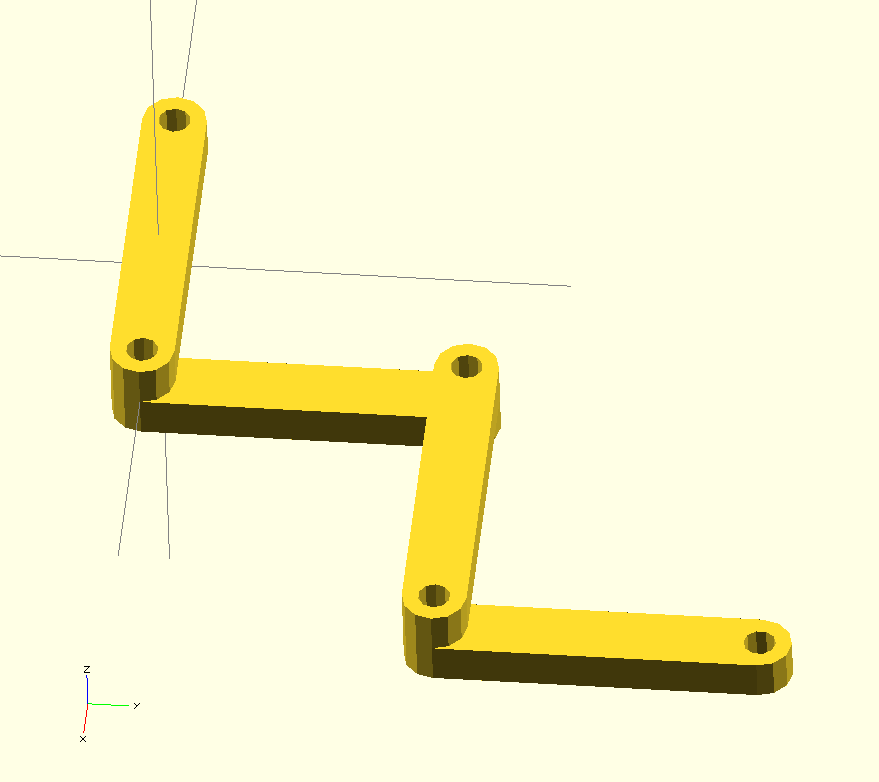
\includegraphics[scale=0.5]{images/image12.png}
	\caption{OpenSCAD View : 4Bar Sample}
	\label{fig:4bar-openscad}
\end{figure}

\subsection{Algorithmic Approach}

The general geometric constraint problem consists of a finite set 
of geometric elements, links, and  a finite set of constraints between them \citep{hoffmann1998gcd}.  
The constraints are logical constraints, such as coincidence, parallelism, etc., 
or metric constraints, such as distance or angle offsets. 
A solution is one where all the constraints are satisfied (not violated). 
Clearly, for a set of constraints there may be a multitude of solutions. 
In general, any geometric constraint problem can be transformed into a set of non-linear equations. 
Solving these systems generally results in algorithms of 
at least exponential time complexity \citep{hoffmann1998gcd} or worse. 
Strict numerical approaches suffer from problems of convergence.  
Even simple problems such as the Figure \ref{fig:two-stick-problem} \citep{kramer1991sgcs}
have convergence issues due to the presence of multiple solutions. 

\begin{figure}[h!]
	\centering
	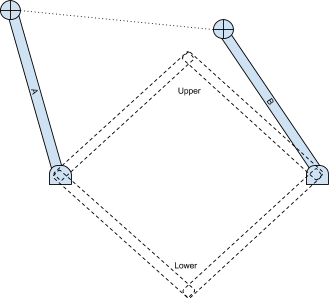
\includegraphics[scale=0.7]{images/image04.png}
	\caption{Two Stick Problem}
	\label{fig:two-stick-problem}
\end{figure}

Equally troublesome are issues of meaning. 
For example, when an under-constrained system produces no solution, 
there is little indication as to the system's deficiencies.
The FLA is based on \citep{kramer1991sgcs} and the approach of solving constraint 
systems by decreasing the degrees-of-freedom, DOF, of the system.  
This approach makes progress by repeatedly making passes over the 
system of constraints so long as the the DOF decreases on the last pass. 
We carefully select specific classes of geometric constraint problems 
which have algorithms with good time complexity. 
It is convenient to notice that the  goal of selecting such 
classes of subproblems, finding dense subgraphs, also represents known best design practice. 
For example, creating rigid joints when feasible is both good design practice 
and a well-solved constraint problem. A key element of this approach 
is that the set of functions is open; 
as additional assembly structures are identified and their 
algorithms specified, the attendant functions can be added 
to the assembly knowledge database, each function with its identifying predicate. 
The problem then reduces to selecting a constraint set, 
with their associated objects, and evaluating the predicates in the knowledge database. 
When a predicate is true, the associated function is evaluated, 
the evaluation resulting in a decreased degrees-of-freedom for the system.  

\subsubsection{Guide Analysis}

Sometimes analysis results in a finite number of solutions 
from which a single solution must be selected. 
These cases are resolved by providing a guide point to the constraint. 
The closest (optionally farthest) solution to the guide is selected. 
This element is not common in commercial CAD where it is presumed that the interactive user will manually select the correct solution from several. 
This conventional approach effectively casts away this critical choice.

\subsubsection{Anchored Analysis}

An anchored constraint is a constraint that has one link that is fully constrained. 
This is a well known sub-problem addressed in \citep{kramer1991sgcs}. 
Assuming a finite number of primitive constraints there are a finite number of functions. 
There are a finite number of functions which reduce 
the degrees-of-freedom for a linkage using these primitive constraints. 
The application of these constraints either leads to a rigid body solution, 
a solution with conflicting constraints, an insufficiently constrained solution, 
or an appropriately underconstrained kinematic solution. 
Of these solutions, some are in need of correction either by adding, 
removing or adjusting the constraint network. 
There is also the potential for there to be constraints that are not applied. 
In this case no function is yet provided. 
If no function is provided, it is possible for the engineer to propose 
and contribute such a function, thereby extending the system and resolving the additional constraints.
The basic set of primitive anchored constraints are defined between two links (e.g. 'A' and 'B'). 
Compounds of these primitive joints are used to describe many lower joints, 
such as revolute, prismatic, screw, cylindrical, fixed, spherical, planar and universal. 
(Higher joints are also composites which are only partially described with primitives.) 
With these primitives, we have the basis for a complexity metric. 
The application of each of these primitives reduces the degrees-of-freedom (DOFs) 
of the system by some small amount which is arbitrarily specified as unity. 
As this is an anchored analysis, only the interaction of the mobile link 
with the fixed link over the primitive needs to be considered. 
As an example, one definition of complexity is as a psychological model 
of the number of atomic ideas the designer needs to consider simultaneously. 
The reduction in the system's degrees-of-freedom associated with the application 
of a primitive provides a metric indicating these atomic ideas. 
A lower joint, such as the revolute-joint, is composed of two primitives 
and reduces the degrees-of-freedom (DOFs) by five, 
the revolute's primitive coincident-point joint and 
parallel-axis-joint reducing the DOFs by three and two respectively.
The primitives may be placed such that the DOFs of the system are not reduced. 
In these cases, they serve to reinforce or contradict the rules 
already applied to the system. 
In the following descriptions of the primitives, 
the number of DOFs typically constrained are indicated.

\paragraph{coincident-point joint}

This constrains all three translational DOFs. 
A point in link A is coincident with a point in link B. 

\begin{figure}[ht!]
	\centering
	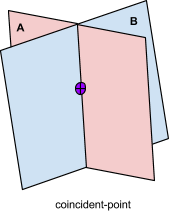
\includegraphics[scale=0.7]{images/image06.png}
	\caption{coincident-point joint primitive}
	\label{fig:coincident-point-primitive}
\end{figure}

\paragraph{in-line joint}

This constrains two translational DOFs. 
A point in link A lies on a line in link B. 

\begin{figure}[ht!]
	\centering
	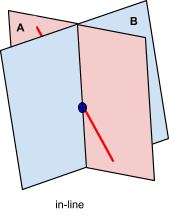
\includegraphics[scale=0.7]{images/image14.png}
	\caption{in-line joint primitive}
    \label{fig:in-line-primitive}
\end{figure}

\paragraph{in-plane joint}

This constrains one translational DOF. 
A point in link A lies on a plane in link B.

\begin{figure}[ht!]
	\centering
	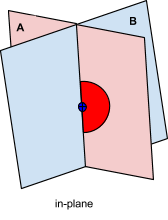
\includegraphics[scale=0.7]{images/image15.png}
	\caption{in-plane joint primitive}
	\label{fig:in-plane-primitive}
\end{figure} 

\paragraph{parallel-axis joint}

This constrains two rotational DOFs. 
A line in link A is parallel to a line on link B. 
Combining the parallel-joint with other primitive joints produces several compound joints: 
with a coincident-joint produces a revolute joint; 
with an in-line-joint produces a cylindrical-joint; 
with an in-plane-joint produces a planar-joint.

\begin{figure}[ht!]
	\centering
	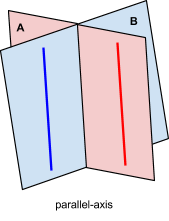
\includegraphics[scale=0.7]{images/image05.png}
	\caption{parallel-axis joint primitive}
	\label{fig:parallel-axis-primitive}
\end{figure}

\paragraph{offset-line joint}

This constrains one rotational DOF. 
Given the coincident-point constraint the angle between a line in A and 
a line in B have a specified magnitude. 
When the angle is zero the parallel-axis constraint is used.

\begin{figure}[ht!]
	\centering
	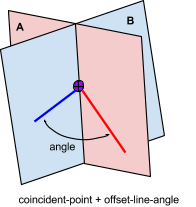
\includegraphics[scale=0.7]{images/image01.png}
	\caption{offset-line joint primitive}
	\label{fig:offset-line-primitive}
\end{figure} 
 

\paragraph{offset-plane joint}

This constrains one rotational DOF. 
Given the parallel-axis constraint, there are planes in A and B 
containing the parallel lines such that the angle between them is a measured value. 

\begin{figure}[h!]
	\centering
	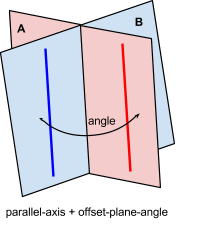
\includegraphics[scale=0.7]{images/image09.png}
	\caption{offset-plane joint primitive}
	\label{fig:offset-plane-primitive}
\end{figure}

\paragraph{helical joint}

This fuses two rotational DOFs into one helical DOF. 
Given an in-line and a parallel-axis constraint, 
the offset-plane-angle is linearly related to the position of 
the in-line point along that line. 
The helical constraint binds a rotational DOF to a translational DOF. 
Two notable examples are the screw and the rolling wheel, 
but there are other less obvious cases. 

%% \begin{figure}[ht!]
%%	\centering
%%	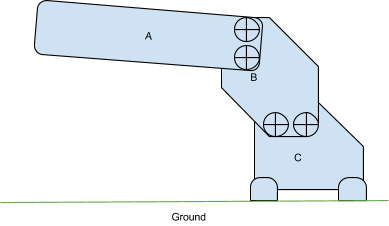
\includegraphics[scale=0.7]{images/image16.png}
%%	\caption{helical joint primitive}
%%	\label{fig:helical-primitive}
%% \end{figure}

\subsubsection{Binary Locus Analysis}

A strict binary constraint is one where each link is 
partially constrained and which together allow the candidate constraint to be satisfied unambiguously. 
The two-stick problem presented previously is a representative example. 
In the two-stick problem there are two valid solutions, 
one of the multiple solutions is selected by providing a guide constraint. 
The binary locus analysis and resulting joint is 
more complex than that obtained by anchor analysis. 
Indeed, the constraint must be considered twice as the two links mutually position each other. 
The guide needed for a single solution increases the complexity by at least one.

\subsubsection{n-ary Locus Construction}

This is the general case where a set of links is partially 
constrained and the constraint can be satisfied by producing a set of solution candidates, a locus. 
The formation of such a locus can be considered a 
fractional reduction in the DOFs of the participating links. 
These linkage assemblies accumulate complexity toward 
a final assembly where all potential interactions, 
a complete subgraph (clique), between participating links need to be considered. 
These have complexity O(n2). In some severe cases, 
the constraints interact with each other as well as their links, 
resulting in $O(2^n)$ time complexity. 
Ultimately, each DOF reducing function must be carefully 
considered to decide how many interactions are in play. 
Consider the two figures which contain the same number of links but different complexities.

\begin{figure}[h!]
	\centering
	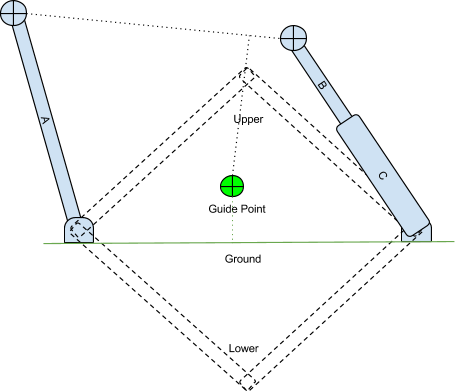
\includegraphics[scale=0.7]{images/image03.png}
	\caption{High Complexity Constraint Application}
	\label{fig:high-complexity}
\end{figure} 

\begin{figure}[h!]
	\centering
	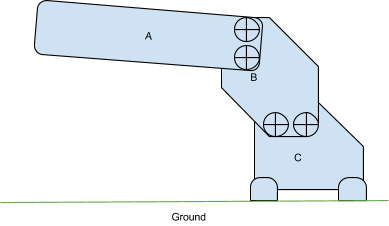
\includegraphics[scale=0.7]{images/image16.png}
	\caption{Low Complexity Constraint Application}
	\label{fig:low-complexity}
\end{figure} 

\subsubsection{Component Construction}

A subset of the total constraint graph has a solution if one of constituent links is assumed to be fixed. 
This is the design practice of component sub-assemblies.
Components provide a means for reducing the complexity of a linkage assembly. This is borne out by the reduction of the number of links considered on the constraint. Once a link becomes rigid, the combinatorial complexity is effectively isolated to the component.

\subsection{Validation} 

FLA is a work in progress following a test-driven development approach. 
A set of problems with characteristics of those problems seen during the AVM projects has been constructed. 
Many of the tests associated with these problems currently pass. 
These include coincident coordinate systems, coincident planes, and coincident points.
 
\subsection{Alternatives/Trade-offs}

One good design practice is to select designs that lend themselves to deterministic solutions. 
This approach is to emphasize constraints having clear analytic solutions. 
An outcome of this approach is the guide constraint being added to obtain unique solutions without ambiguity.
Most interactive CAD systems start with numerical solutions and resolve ambiguities 
with heuristics or special operator input. The approach is to leave 
the development of additional constraint solutions open so that they
may be solved by the larger academic and practicing communities. 
FLA has been developed using technology that allows targeting 
of multiple virtual machines (JVM, .Net, V8), allowing it 
to be used as a library as well as a stand-alone executable. 
The individual functions exist in the public domain, as the relevant patents expired in 2014.

\subsection{Future Enhancements}

The current project, through the introduction of an open-source reference implementation, 
has demonstrated the capability to generate input for additional visualizers. 
Work has already begun to produce input for BRL-CAD, FreeCAD and cad.js \footnote{\url{https://github.com/ghemingway/cad.js}}. 
Compatible proprietary visualizers are welcome.

\subsubsection{Collaborative Design}

The components for the \texttt{CAD\_Assembly.xml} are now set up so that each component 
with associated transform and constraints are atomic, so that the order is no longer important; 
these make it possible to add or delete constraints and components asynchronously. 
This asynchrony provides the basis for support of  \url{http://en.wikipedia.org/wiki/Cloud-based_design_and_manufacturing} (CBDM).
The tools thus developed serve as a high level abstraction 
for performing "skeleton design". 
In skeleton design, work is partitioned among workers in a collaborative fashion. 
Studies have shown that such partitioning is critical to effective collaboration to eliminate conflicts.
%% todo cite the studies  
The current environment for FLA is synchronous batch, but 
the tool is capable of being placed in an asynchronous distributed 
collaborative environment such as that enabled by the Meta-Link Exchange.

\begin{figure}[h]
\centering
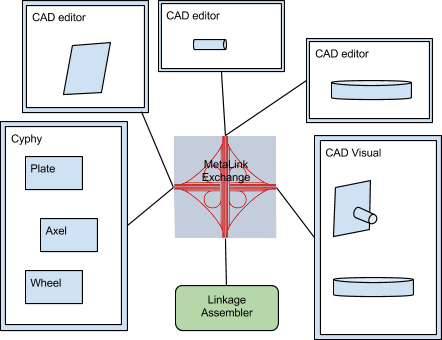
\includegraphics[width=0.7\linewidth]{images/image08}
\caption[Asynchronous METALink Federation]{METALink Enabled Asynchronous Federated Environment}
\label{fig:async-metalink}
\end{figure}


\subsubsection{Kinematics}

A successful run of FLA discovers a linkage assembly plan. 
This assembly plan is not presently written as an output from FLA, 
but would be useful input to a kinematic solver.

\subsubsection{Complexity Metrics}

The linkage assembly plan is an artifact produced by the linkage assembler. 
It is susceptible to several types of analysis, including assembly robustness, 
assembly composability, component discovery, and design resilience. 
As more complex designs are developed, new functions may need to be written to properly assemble them. 
Because this is an open-source assembler, the set of assembly functions is an open set; 
new functions can be added to FLA. 
These assembly functions represent distinct structural designs, 
each with their own complexity metric. 
The assembly complexity for a linkage is a norm over these component complexities. 
These structural designs can be studied and evaluated.

\begin{figure}[h!]
	\centering
	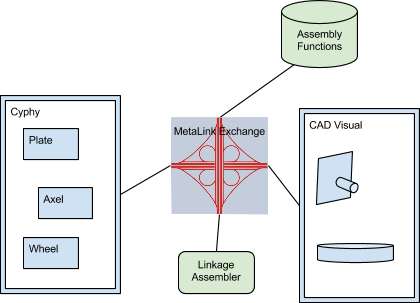
\includegraphics[scale=0.7]{images/image17.png}
	\caption{Federated Assembly Functions}
	\label{fig:federated-metalink}
\end{figure}

\subsection{AVM Involvement}

This is a fairly late entry to the project, so it was not available for AVM testing.  
Even though enough capabilities are available to have been used for AVM, it is still in an early phase of development.

\subsection{Summary/Conclusion} 

\blockquote[Paul Eremenko]{
The substantial time advantage which stands to be gained from META and iFAB is 
predicated on the existence of detailed models of components, of the environment (contexts),
and of manufacturing equipment and processes. 
This requires significantly more information than exists in most present-day component models, 
which are typically little more than performance curves and interface specifications...}.
 
The development of a linkage assembler that can assemble 
common-off-the-shelf  (“catalog”), parametric (“rubber”), and 
theoretical (“ghost”) components is critical to improving systems engineering 
on the functional deployment side of the systems engineering process. 
The development of the freed-linkage-assembler (FLA) demonstrates that it is 
possible to visualize assemblies without a proprietary compositional assembler. 
OpenMETA is extended with a simple island grammar which provides constraint port descriptions.  
In CyPhy these ports may be joined to form fixed and kinematic joints. 
Composition of assemblies with fixed joints is currently supported, while kinematic joint construction from constraints is ongoing.

\chapter{Federation}

\epigraph{The public good is in nothing more essentially interested, 
than in the protection of every individual's private rights.}{William Blackstone}


%% something about sandstorm, webgme, assembly plan graph analysis.

\chapter{Implementation}

%% something about extension of the system by federation partners

\chapter{Complexity}

%% what are the types of complexity analysis that can be done
%% given an assembly plan graph.

\chapter{Kinematics}

%% inverse kinematics, interferance studies, dynamic forces.

	
	\bibliographystyle{plain}
	\bibliography{references}
	
\end{document} 